\documentclass[
11pt, % The default document font size, options: 10pt, 11pt, 12pt
%codirector, % Uncomment to add a codirector to the title page
]{charter} 




% El títulos de la memoria, se usa en la carátula y se puede usar el cualquier lugar del documento con el comando \ttitle
\titulo{Sistema de monitoreo de un equipo de extracción de petróleo} 

% Nombre del posgrado, se usa en la carátula y se puede usar el cualquier lugar del documento con el comando \degreename
%\posgrado{Carrera de Especialización en Sistemas Embebidos} 
\posgrado{Carrera de Especialización en Internet de las Cosas} 
%\posgrado{Carrera de Especialización en Intelegencia Artificial}
%\posgrado{Maestría en Sistemas Embebidos} 
%\posgrado{Maestría en Internet de las cosas}

% Tu nombre, se puede usar el cualquier lugar del documento con el comando \authorname
\autor{Ing. Eduardo Agustín Sciutto} 

% El nombre del director y co-director, se puede usar el cualquier lugar del documento con el comando \supname y \cosupname y \pertesupname y \pertecosupname
\director{Mag. Ing. Adrián S. Nowik}
\pertenenciaDirector{UP/PAE} 
% FIXME:NO IMPLEMENTADO EL CODIRECTOR ni su pertenencia
\codirector{John Doe} % para que aparezca en la portada se debe descomentar la opción codirector en el documentclass
\pertenenciaCoDirector{FIUBA}

% Nombre del cliente, quien va a aprobar los resultados del proyecto, se puede usar con el comando \clientename y \empclientename
\cliente{Ing. Nicolás D. Brunini}
\empresaCliente{PAE}

% Nombre y pertenencia de los jurados, se pueden usar el cualquier lugar del documento con el comando \jurunoname, \jurdosname y \jurtresname y \perteunoname, \pertedosname y \pertetresname.
\juradoUno{Nombre y Apellido (1)}
\pertenenciaJurUno{pertenencia (1)} 
\juradoDos{Nombre y Apellido (2)}
\pertenenciaJurDos{pertenencia (2)}
\juradoTres{Nombre y Apellido (3)}
\pertenenciaJurTres{pertenencia (3)}
 
\fechaINICIO{21 de junio de 2022}		%Fecha de inicio de la cursada de GdP \fechaInicioName
\fechaFINALPlan{9 de agosto de 2022} 	%Fecha de final de cursada de GdP
\fechaFINALTrabajo{21 de junio de 2023}	%Fecha de defensa pública del trabajo final


\begin{document}

\maketitle
\thispagestyle{empty}
\pagebreak


\thispagestyle{empty}
{\setlength{\parskip}{0pt}
\tableofcontents{}
}
\pagebreak


\section*{Registros de cambios}
\label{sec:registro}


\begin{table}[ht]
\label{tab:registro}
\centering
\begin{tabularx}{\linewidth}{@{}|c|X|c|@{}}
\hline
\rowcolor[HTML]{C0C0C0} 
Revisión & \multicolumn{1}{c|}{\cellcolor[HTML]{C0C0C0}Detalles de los cambios realizados} & Fecha      \\ \hline
0      & Creación del documento                                 &\fechaInicioName \\ \hline
1      & Se completa hasta el punto 5 inclusive                 & 2 de julio de 2022 \\ \hline
2      & Se completa hasta el punto 9 inclusive					& 9 de julio de 2022 \\
\hline
%		  Se puede agregar algo más \newline
%		  En distintas líneas \newline
%		  Así                                                    & dd/mm/aaaa \\ \hline
%3      & Se completa hasta el punto 11 inclusive                & dd/mm/aaaa \\ \hline
%4      & Se completa el plan	                                 & dd/mm/aaaa \\ \hline
\end{tabularx}
\end{table}

\pagebreak



\section*{Acta de constitución del proyecto}
\label{sec:acta}

\begin{flushright}
Buenos Aires, \fechaInicioName
\end{flushright}

\vspace{2cm}

Por medio de la presente se acuerda con el Ing. \authorname\hspace{1px} que su Trabajo Final de la \degreename\hspace{1px} se titulará ``\ttitle'', consistirá esencialmente en la implementación de un prototipo de un sistema de monitoreo de un equipo de extracción de petróleo, y tendrá un presupuesto preliminar estimado de 600 hs de trabajo y ARS 650.000,00, con fecha de inicio \fechaInicioName\hspace{1px} y fecha de presentación pública \fechaFinalName.

Se adjunta a esta acta la planificación inicial.

\vfill

% Esta parte se construye sola con la información que hayan cargado en el preámbulo del documento y no debe modificarla
\begin{table}[ht]
\centering
\begin{tabular}{ccc}
\begin{tabular}[c]{@{}c@{}}Dr. Ing. Ariel Lutenberg \\ Director posgrado FIUBA\end{tabular} & \hspace{2cm} & \begin{tabular}[c]{@{}c@{}}\clientename \\ \empclientename \end{tabular} \vspace{2.5cm} \\ 
\multicolumn{3}{c}{\begin{tabular}[c]{@{}c@{}} \supname \\ Director del Trabajo Final\end{tabular}} \vspace{2.5cm} \\
%\begin{tabular}[c]{@{}c@{}}\jurunoname \\ Jurado del Trabajo Final\end{tabular}     &  & \begin{tabular}[c]{@{}c@{}}\jurdosname\\ Jurado del Trabajo Final\end{tabular}  \vspace{2.5cm}  \\
%\multicolumn{3}{c}{\begin{tabular}[c]{@{}c@{}} \jurtresname\\ Jurado del Trabajo Final\end{tabular}} \vspace{.5cm}                                                                     
\end{tabular}
\end{table}




\section{1. Descripción técnica-conceptual del proyecto a realizar}
\label{sec:descripcion}


% El bloque "consigna" se usa para poner texto en rojo y dar una pequeña ayuda sobre cómo completar la sección

La gestión eficiente de un yacimiento productor de petróleo no electrificado y de periferia plantea grandes desafíos. El modelo de operación usualmente se basa en la presencia diaria de cuadrillas de operarios cuya principal función es recorrer cada instalación y realizar un relevamiento funcional. Excepcionalmente, ejecutan alguna tarea correctiva en función de lo identificado en la visita.
En la actualidad, existen zonas donde los aparatos individuales de bombeo (AIB) no disponen de supervisión remota dado que originalmente la implementación de una solución tradicional de telemetría fue considerada económicamente inviable. La principal razón, es el costo de proveer un sistema alternativo de energía confiable para dicho equipamiento que generalmente está basado en paneles solares y baterías. Otra consideración es el riesgo de sabotaje y robo de equipamiento de medición costoso en zonas alejadas y con vigilancia deficiente. 

El hecho de que un AIB deje de funcionar de manera imprevista, afecta directamente la producción de petróleo, por lo que resulta de valor disponer de una alerta inmediata ante dicha situación. Además, la información histórica de los períodos de tiempo de no funcionamiento facilita y hace más precisa la elaboración del informe de down-time por parte de los supervisores de producción.
 
Recientemente, la empresa operadora del yacimiento implementó una red LoRaWAN propia con extensa cobertura en el yacimiento. Sintéticamente, LoRaWAN es una tecnología de comunicación inalámbrica bidireccional, que hace posible administrar muchos nodos alimentados a baterías (con vida útil típica de varios años) conectados hasta varios kilómetros de distancia y transmitiendo a una muy baja tasa de datos (decenas de bytes pocas veces al día). Estas características hacen viable una implementación de internet de las cosas industrial (IIoT) para el caso mencionado, resaltando el aporte de mayor eficiencia y de reducción de costos operativos.

Otro aspecto para considerar es el de buscar una solución de rápida implementación y de mayor flexibilidad ante cambios, que aporte información relevante a los usuarios finales. Implementar un sistema de SCADA con tecnología tradicional es un trabajo complejo y demandante de tiempo, requiere la intervención de profesionales de distintos sectores dentro de la empresa ya que involucra tareas de configuración, calibración y enrutamiento en distintos sistemas on-premise. En muchos casos es justificada su utilización dada la criticidad e importancia de los procesos que se controlan y monitorean. Por otro lado, se ve una oportunidad en la utilización de distintos servicios en la nube, principalmente para procesar fuentes de datos no críticos que complementan o brindan nueva información de variables de campo y que se adaptan fácilmente a los cambios en las necesidades de visualización y notificación de los usuarios finales.

El objeto del presente proyecto es el desarrollo de una solución de monitoreo y alarmas de bajo costo para equipos AIB de un yacimiento de periferia. Se utilizarán una red LoRaWAN y componentes en la nube de Microsoft Azure.
En particular, se implementará un prototipo que medirá el estado funcional del AIB. El servidor de red LoRaWAN canalizará la información generada por el sensor a un grupo de recursos creados en la nube de Microsoft Azure mediante el protocolo AMQP.
En la nube se realizarán diferentes procesos, que contemplan la decodificación de la información, almacenamiento en base de datos y utilización de una aplicación back end que administrará el acceso a información estadística y la notificación de alertas a los usuarios autorizados.
Los usuarios dispondrán de al menos un tipo de front end para el consumo de la información.

En la figura \ref{fig:diagBloques} se presenta el diagrama en bloques del sistema descripto.

%\vspace{25px}

\begin{figure}[htpb]
\centering 
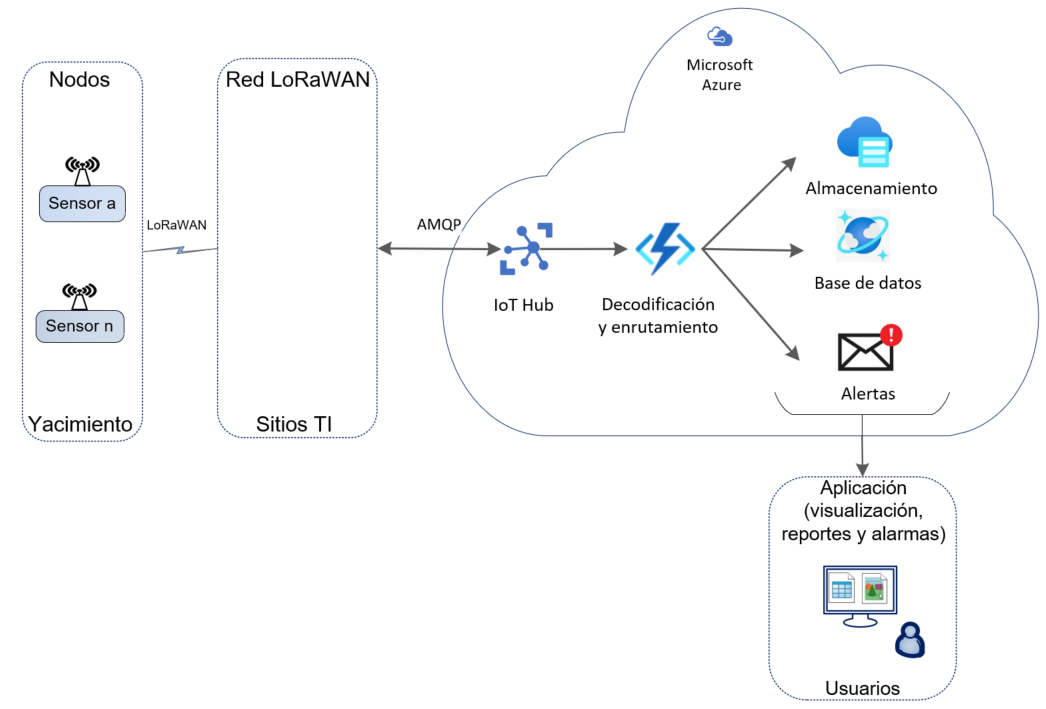
\includegraphics[width=.8\textwidth]{./Figuras/diagrama_bloques_conceptual2.png}
\caption{Diagrama en bloques del sistema}
\label{fig:diagBloques}
\end{figure}

\vspace{25px}




\section{2. Identificación y análisis de los interesados}
\label{sec:interesados}


\begin{table}[ht]
%\caption{Identificación de los interesados}
%\label{tab:interesados}
\begin{tabularx}{\linewidth}{@{}|l|X|X|l|@{}}
\hline
\rowcolor[HTML]{C0C0C0} 
Rol           & Nombre y Apellido & Organización 	& Puesto 	\\ \hline
Auspiciante   & Juan A. Aranguren & \empclientename & Exec. Manager TEC-IT       	\\ \hline
Cliente       & \clientename      &\empclientename &  Leader UPO-OP II D5      	\\ \hline
Impulsor      & Eduardo O. Domínguez                  &\empclientename & Exec. Manager IT Regional       	\\ \hline
Responsable   & \authorname       &\empclientename        	& SR Specialist TEC-IT 	\\ \hline
Colaboradores & Gustavo G. Conrad \newline 
				Germán Gornatti					&\empclientename             	& Specialist TEC-IT  \\ \hline
%			& Germán Gornatti &\empclientename & SR Engineer UPO-Control Engineering     \\ \hline
Orientador    & \supname	      & \pertesupname 	& Director Trabajo final \\ \hline
%Equipo        & miembro1 \newline 
%				miembro2          &              	&        	\\ \hline
Opositores    &  Sector de OT                 &  \empclientename            	&   USP-OP     	\\ \hline
Usuario final & Nestor O. Bochatey  & \empclientename             	& Field Foreman UPO-OP II D5       	\\ \hline
\end{tabularx}
\end{table}

A continuación se listan las principales características de cada interesado.

\begin{itemize}
	\item Auspiciante: muy interesado en que la implementación resulte exitosa y sirva de modelo para nuevos desarrollos.
	\item Cliente: desea obtener resultados en corto tiempo. Se debe tener riguroso seguimiento del plan de trabajo acordado.
	\item Colaboradores: su dedicación a este proyecto es de tiempo parcial y no está reflejada en los objetivos de desempeño con sus gerencias funcionales. Se debe trabajar en sostener la motivación.
	\item Orientador: profesional de alta capacidad técnica y de gestión. Tener muy en cuenta sus observaciones.
	\item Usuario final: desde el inicio mantener un vínculo estrecho y capacitarlo adecuadamente en el uso de las nuevas herramientas. Buscar de convertirlo en un aliado.
	\item Opositores: el desarrollo del proyecto puede afectar intereses y actual metodología de trabajo del equipo de tecnología operacional (TO).
\end{itemize}




\section{3. Propósito del proyecto}
\label{sec:proposito}

El propósito de este proyecto es impulsar la aplicación de nuevas tecnologías en la industria del petróleo y gas. Se busca implementar un sistema de monitoreo y alertas, utilizando una arquitectura típica de IIoT, para casos donde un sistema tradicional de telemetría no ha resultado económicamente viable.


\section{4. Alcance del proyecto}
\label{sec:alcance}

El alcance del trabajo final incluye los siguientes aspectos.

\begin{itemize}
\item Adaptación de un nodo comercial LoRaWAN para detectar el estado de Marcha/Parada del motor de un AIB. Opcionalmente se evaluará incorporar otra variable física de tipo analógica, por ejemplo, vibración. Se busca realizar la selección, la integración y el ensayo del conjunto nodo más transductores.

\item Conexión entre el servidor de red LoRaWAN y el componente IoT Hub de Microsoft Azure en la nube, utilizando el protocolo MQTT o AMQP.

\item Decodificación de la carga útil de los mensajes enviados por los sensores. Filtrado y almacenamiento de información relevante en una base de datos.

\item Creación de una aplicación de servidor y de una aplicación de interfaz de usuario para gestionar y entregar información de monitoreo y alarmas a los usuarios finales.

\end{itemize}

No se incluye en el alcance del proyecto lo siguiente.

\begin{itemize}

\item Estudios de confiabilidad y análisis de fallas relacionados al mantenimiento predictivo del prototipo a implementar.

\item Arquitectura y configuración de la red LoRaWAN que da servicio de conexión de los sensores.

\end{itemize}



\section{5. Supuestos del proyecto}
\label{sec:supuestos}

Para el desarrollo del presente proyecto se asume lo siguiente.

\begin{itemize}
\item Se contará con el hardware y materiales necesarios para implementar los prototipos de medición. Además, se autorizará el alta de los mismos a la red LoRaWAN existente.
\item Se tendrá acceso y apoyo de personal calificado para instalar y manipular los prototipos de medición en un grupo de AIB operativos del yacimiento.
\item Se dispondrá de una suscripción activa a un grupo de recursos para implementar todos los componentes de la solución en la nube de Microsoft Azure.
\item Existirán acuerdos y aprobaciones de los sectores de Seguridad Informática y Tecnología Operacional para establecer las conexiones de datos entre los componentes de la solución.

\end{itemize}


\section{6. Requerimientos}
\label{sec:requerimientos}
%\begin{consigna}{red}
Se presentan a continuación los requerimientos del proyecto.
\begin{enumerate}
	\item Requerimientos asociados al dispositivo de medición.
		\begin{enumerate}
			\item No debe requerir mano de obra calificada, tanto para la instalación como para la operación cotidiana.
			\item Debe ser robusto y soportar condiciones de clima extremo (grado de protección IP 67, soportar temperaturas entre -20°C y 50°C).
			\item Debe funcionar con baterías internas y poseer una autonomía de al menos 3 años.
			\item La batería debe ser comercialmente asequible y de fácil reemplazo.
			\item El estado e información de los sensores del dispositivo se deben poder consultar mediante una aplicación inalámbrica desde un celular y de forma sencilla.
			\item Debe permitir el traslado a una nueva ubicación sin requerir una reconfiguración local.
			\item Debe detectar y notificar de forma inmediata si un sensor tiene una falla de cableado.
		\end{enumerate}
		
	\item Requerimientos asociados a la colecta e identificación de mensajes generados por los dispositivos.
		\begin{enumerate}
			\item Se deberá definir un nomenclador de tópicos que sea flexible y escalable.
			\item La estructura de la carga útil del mensaje debe soportar futuras  incorporaciones de sensores.
		\end{enumerate}

	\item Requerimientos asociados al software en la nube.
		\begin{enumerate}
			\item Se deberán utilizar componentes de la plataforma Azure de Microsoft.
			\item Los mensajes de los dispositivos se enviarán a un componente IoT Hub mediante protocolo AMQP.
			\item Se deberá decodificar y enrutar adecuadamente el flujo de datos proveniente de IoT Hub.
			\item Se debe establecer un flujo de datos hacia una base de datos de históricos.
			\item Se debe establecer un flujo de datos para procesar y enviar notificaciones de alarmas.
			\item Se deberá definir un mecanismo de notificación de alarmas y eventos a los usuarios registrados. Podrá ser por email y/o Telegram.
			\item La aplicación web dispondrá de un panel para visualizar información histórica de cada dispositivo.
			\item La aplicación web permitirá la consulta de eventos y alarmas.
Se debe recibir una notificación de forma inmediata ante un paro del motor.
			\item Se deben recibir notificaciones de advertencia de nivel de batería bajo y algún otro parámetro que se identifique de utilidad, para realizar un correcto mantenimiento preventivo.
		\end{enumerate}

	\item Requerimientos de integridad y seguridad.
		\begin{enumerate}
			\item Se deberá establecer un mecanismo seguro de gestión y validación de usuarios de la aplicación web.
			\item El acceso a la configuración de los dispositivos de medición estará protegido por un usuario y contraseña. Será utilizado únicamente por personal autorizado del sector TI de la empresa.
		\end{enumerate}
	
	\item Requerimientos de documentación.
		\begin{enumerate}
			\item Se deberá elaborar el manual de configuración e instalación del dispositivo de medición.			
			\item Se deberá documentar la configuración de todos los componentes desplegados en Microsoft Azure.
			\item Se deberá elaborar el manual de uso del software de usuario.
			\item Se deberá desarrollar el informe de avance del proyecto.
			\item Se deberá desarrollar la memoria final del proyecto.
		\end{enumerate}
		
	\end{enumerate}



\section{7. Historias de usuarios (\textit{Product backlog})}
\label{sec:backlog}

%\begin{consigna}{red}
%Descripción: En esta sección se deben incluir las historias de usuarios y su ponderación (\textit{history points}). Recordar que las historias de usuarios son descripciones cortas y simples de una característica contada desde la perspectiva de la persona que desea la nueva capacidad, generalmente un usuario o cliente del sistema. La ponderación es un número entero que representa el tamaño de la historia comparada con otras historias de similar tipo.
%
%El formato propuesto es: "como [rol] quiero [tal cosa] para [tal otra cosa]."
%
%Se debe indicar explícitamente el criterio para calcular los \textit{story points} de cada historia
%\end{consigna}
Para la elaboración de historias de usuario se definió un índice de ponderación compuesto por la suma de tres propiedades: dificultad, complejidad e incertidumbre o riesgo. Cada propiedad es cuantificada mediante la serie de Fibonacci (0, 1, 2, 3, 5, 8, 13, …) adoptándose el siguiente criterio que aplica a las tres propiedades por igual.
\begin{itemize}
\item Valores: 0, 1, 2 es una cuantificación baja.
\item Valores: 3 y 5 es una cuantificación media.
\item Valores: 8 o superior es una cuantificación alta.
\end{itemize}

A continuación, se detallan las historias de usuario recopiladas.

\begin{itemize}

\item Como supervisor de producción quiero ser notificado de la parada de un AIB de inmediato para poder enviar una cuadrilla y minimizar el downtime. Ponderación: 12 (dificultad: 5, complejidad: 5, riesgo: 2).

\item Como supervisor de producción quiero tener acceso a una pantalla sencilla que me muestre el estado histórico de un AIB para poder calcular fácilmente el downtime. Ponderación: 10 (dificultad: 5, complejidad: 3, riesgo: 2).

\item Como supervisor de producción deseo recibir las notificaciones importantes en mi celular para tener mejor tiempo de respuesta, ya que no siempre estoy en la oficina. Ponderación: 16 (dificultad: 8, complejidad: 5, riesgo: 3).

\item Como encargado de mantenimiento quiero tener información frecuente del estado de carga de las baterías para programar eficientemente las tareas de las cuadrillas del sector. Ponderación: 6 (dificultad: 2, complejidad: 3, riesgo: 1).

\item Como jefe de distrito quiero que mis colaboradores optimicen sus salidas al campo para poder dedicar más tiempo a tareas analíticas en la oficina. Ponderación: 12 (dificultad: 5, complejidad: 5, riesgo: 2).

\item Como jefe de distrito quiero minimizar el uso de las horas de cuadrilla para poder reducir costos operativos. Ponderación: 12 (dificultad: 5, complejidad: 5, riesgo: 2).

\item Como referente de TI quiero que la aplicación solo la puedan utilizar usuarios autorizados para preservar la confidencialidad e integridad de los datos. Ponderación: 11 (dificultad: 3, complejidad: 5, riesgo: 3).

\item Como referente de TI quiero democratizar el acceso a la información para que nuevos usuarios puedan aportar más valor a sus tareas. Ponderación: 12 (dificultad: 5, complejidad: 2, riesgo: 5).

\item Como desarrollador de la aplicación quiero armar un sistema flexible y escalable para incorporar nuevas funcionalidades en el futuro. Ponderación: 15 (dificultad: 5, complejidad: 5, riesgo: 5).
\end{itemize}

\section{8. Entregables principales del proyecto}
\label{sec:entregables}

%\begin{consigna}{red}

Los entregables del proyecto son:

\begin{itemize}
	\item Diagrama esquemático del dispositivo de medición.
	\item Manual de configuración e instalación del dispositivo de medición.
	\item Documentación de configuración de componentes en Microsoft Azure.
	\item Código fuente del software de usuario.
	\item Manual de uso del software de usuario.
	\item Informe de avance del proyecto.
	\item Memoria final del proyecto.
\end{itemize}

%\end{consigna}

\section{9. Desglose del trabajo en tareas}
\label{sec:wbs}


\begin{enumerate}
\item Planificación de proyecto. (86 hs)
	\begin{enumerate}
	\item Definición de la arquitectura de la solución. (8 hs)
	\item Investigación de componentes principales del sistema. (40 hs)
	\item Estimación de recursos necesarios y costos asociados. (8 hs)
	\item Definiciones de alcances, requerimientos y presupuestos. (30 hs)
	\end{enumerate}
\item Desarrollo del dispositivo de medición. (130 hs)
	\begin{enumerate}
	\item Análisis y definición de funcionalidades. (4 hs)
	\item Selección de componentes. (18 hs)
	\item Análisis y definición del procedimiento de montaje en el AIB. (20 hs)
	\item Estudio, pruebas y definición de configuración del nodo LoRaWAN. (16 hs)
	\item Análisis, pruebas y definición de transductores. (32 hs)
	\item Integración y pruebas del conjunto nodo - transductores en AIB operativo. (40 hs)
	\end{enumerate}
\item Estructura de mensajes. (42 hs)
	\begin{enumerate}
	\item Definición de jerarquía de tópicos. (18 hs)
	\item Decodificación y escalado de carga útil. (24 hs)
	\end{enumerate}
	
\item Desarrollo de componentes en la nube. (178 hs)
	\begin{enumerate}
	\item Despliegue y configuración del componente IoT Hub. (12 hs)
	\item Despliegue y configuración de la base de datos. (24 hs)
	\item Despliegue y configuración de funciones y flujo de notificaciones. (32 hs)
	\item Despliegue y configuración de componentes para la aplicación del servidor. (40 hs)
	\item Desarrollo de la interfaz de la aplicación de usuario. (40 hs)
	\item Desarrollo de la interfaz para notificaciones por Telegram. (30 hs)
	\end{enumerate}

\item Pruebas de Integración del sistema. (30 hs)
	\begin{enumerate}
	\item Diseño y despliegue de pruebas de funcionalidad integral. (30 hs)
	\end{enumerate}

\item Documentación. (148 hs)
	\begin{enumerate}
	\item Elaboración del informe de avance del proyecto. (30 hs)
	\item Elaboración del manual de configuración e instalación del dispositivo de medición. (24 hs)
	\item Elaboración de la documentación de configuración de componentes en Microsoft Azure. (24 hs)
	\item Elaboración del manual de uso del software de usuario. (24 hs)
	\item Elaboración del informe final del proyecto. (40 hs)
	\item Cierre del proyecto. (6 hs)
	\end{enumerate}
	
\end{enumerate}

Cantidad total de horas: (614 hs)



\section{10. Diagrama de Activity On Node}
\label{sec:AoN}

\begin{consigna}{red}
Armar el AoN a partir del WBS definido en la etapa anterior. 

%La figura \ref{fig:AoN} fue elaborada con el paquete latex tikz y pueden consultar la siguiente referencia \textit{online}:

%\url{https://www.overleaf.com/learn/latex/LaTeX_Graphics_using_TikZ:_A_Tutorial_for_Beginners_(Part_3)\%E2\%80\%94Creating_Flowcharts}

\end{consigna}

\begin{figure}[htpb]
\centering 
\includegraphics[width=.8\textwidth]{./Figuras/AoN.png}
\caption{Diagrama en \textit{Activity on Node}}
\label{fig:AoN}
\end{figure}

Indicar claramente en qué unidades están expresados los tiempos.
De ser necesario indicar los caminos semicríticos y analizar sus tiempos mediante un cuadro.
Es recomendable usar colores y un cuadro indicativo describiendo qué representa cada color, como se muestra en el siguiente ejemplo:



\section{11. Diagrama de Gantt}
\label{sec:gantt}

\begin{consigna}{red}

Existen muchos programas y recursos \textit{online} para hacer diagramas de gantt, entre los cuales destacamos:

\begin{itemize}
\item Planner
\item GanttProject
\item Trello + \textit{plugins}. En el siguiente link hay un tutorial oficial: \\ \url{https://blog.trello.com/es/diagrama-de-gantt-de-un-proyecto}
\item Creately, herramienta online colaborativa. \\\url{https://creately.com/diagram/example/ieb3p3ml/LaTeX}
\item Se puede hacer en latex con el paquete \textit{pgfgantt}\\ \url{http://ctan.dcc.uchile.cl/graphics/pgf/contrib/pgfgantt/pgfgantt.pdf}
\end{itemize}

Pegar acá una captura de pantalla del diagrama de Gantt, cuidando que la letra sea suficientemente grande como para ser legible. 
Si el diagrama queda demasiado ancho, se puede pegar primero la ``tabla'' del Gantt y luego pegar la parte del diagrama de barras del diagrama de Gantt.

Configurar el software para que en la parte de la tabla muestre los códigos del EDT (WBS).\\
Configurar el software para que al lado de cada barra muestre el nombre de cada tarea.\\
Revisar que la fecha de finalización coincida con lo indicado en el Acta Constitutiva.

En la figura \ref{fig:gantt}, se muestra un ejemplo de diagrama de gantt realizado con el paquete de \textit{pgfgantt}. En la plantilla pueden ver el código que lo genera y usarlo de base para construir el propio.

\begin{figure}[htbp]
\begin{center}
\begin{ganttchart}{1}{12}
  \gantttitle{2020}{12} \\
  \gantttitlelist{1,...,12}{1} \\
  \ganttgroup{Group 1}{1}{7} \\
  \ganttbar{Task 1}{1}{2} \\
  \ganttlinkedbar{Task 2}{3}{7} \ganttnewline
  \ganttmilestone{Milestone o hito}{7} \ganttnewline
  \ganttbar{Final Task}{8}{12}
  \ganttlink{elem2}{elem3}
  \ganttlink{elem3}{elem4}
\end{ganttchart}
\end{center}
\caption{Diagrama de gantt de ejemplo}
\label{fig:gantt}
\end{figure}


\begin{landscape}
\begin{figure}[htpb]
\centering 
\includegraphics[height=.85\textheight]{./Figuras/Gantt-2.png}
\caption{Ejemplo de diagrama de Gantt rotado}
\label{fig:diagGantt}
\end{figure}

\end{landscape}

\end{consigna}


\section{12. Presupuesto detallado del proyecto}
\label{sec:presupuesto}

\begin{consigna}{red}
Si el proyecto es complejo entonces separarlo en partes:
\begin{itemize}
	\item Un total global, indicando el subtotal acumulado por cada una de las áreas.
	\item El desglose detallado del subtotal de cada una de las áreas.
\end{itemize}

IMPORTANTE: No olvidarse de considerar los COSTOS INDIRECTOS.

\end{consigna}

\begin{table}[htpb]
\centering
\begin{tabularx}{\linewidth}{@{}|X|c|r|r|@{}}
\hline
\rowcolor[HTML]{C0C0C0} 
\multicolumn{4}{|c|}{\cellcolor[HTML]{C0C0C0}COSTOS DIRECTOS} \\ \hline
\rowcolor[HTML]{C0C0C0} 
Descripción &
  \multicolumn{1}{c|}{\cellcolor[HTML]{C0C0C0}Cantidad} &
  \multicolumn{1}{c|}{\cellcolor[HTML]{C0C0C0}Valor unitario} &
  \multicolumn{1}{c|}{\cellcolor[HTML]{C0C0C0}Valor total} \\ \hline
 &
  \multicolumn{1}{c|}{} &
  \multicolumn{1}{c|}{} &
  \multicolumn{1}{c|}{} \\ \hline
 &
  \multicolumn{1}{c|}{} &
  \multicolumn{1}{c|}{} &
  \multicolumn{1}{c|}{} \\ \hline
\multicolumn{1}{|l|}{} &
   &
   &
   \\ \hline
\multicolumn{1}{|l|}{} &
   &
   &
   \\ \hline
\multicolumn{3}{|c|}{SUBTOTAL} &
  \multicolumn{1}{c|}{} \\ \hline
\rowcolor[HTML]{C0C0C0} 
\multicolumn{4}{|c|}{\cellcolor[HTML]{C0C0C0}COSTOS INDIRECTOS} \\ \hline
\rowcolor[HTML]{C0C0C0} 
Descripción &
  \multicolumn{1}{c|}{\cellcolor[HTML]{C0C0C0}Cantidad} &
  \multicolumn{1}{c|}{\cellcolor[HTML]{C0C0C0}Valor unitario} &
  \multicolumn{1}{c|}{\cellcolor[HTML]{C0C0C0}Valor total} \\ \hline
\multicolumn{1}{|l|}{} &
   &
   &
   \\ \hline
\multicolumn{1}{|l|}{} &
   &
   &
   \\ \hline
\multicolumn{1}{|l|}{} &
   &
   &
   \\ \hline
\multicolumn{3}{|c|}{SUBTOTAL} &
  \multicolumn{1}{c|}{} \\ \hline
\rowcolor[HTML]{C0C0C0}
\multicolumn{3}{|c|}{TOTAL} &
   \\ \hline
\end{tabularx}%
\end{table}


\section{13. Gestión de riesgos}
\label{sec:riesgos}

\begin{consigna}{red}
a) Identificación de los riesgos (al menos cinco) y estimación de sus consecuencias:
 
Riesgo 1: detallar el riesgo (riesgo es algo que si ocurre altera los planes previstos de forma negativa)
\begin{itemize}
	\item Severidad (S): mientras más severo, más alto es el número (usar números del 1 al 10).\\
	Justificar el motivo por el cual se asigna determinado número de severidad (S).
	\item Probabilidad de ocurrencia (O): mientras más probable, más alto es el número (usar del 1 al 10).\\
	Justificar el motivo por el cual se asigna determinado número de (O). 
\end{itemize}   

Riesgo 2:
\begin{itemize}
	\item Severidad (S): 
	\item Ocurrencia (O):
\end{itemize}

Riesgo 3:
\begin{itemize}
	\item Severidad (S): 
	\item Ocurrencia (O):
\end{itemize}


b) Tabla de gestión de riesgos:      (El RPN se calcula como RPN=SxO)

\begin{table}[htpb]
\centering
\begin{tabularx}{\linewidth}{@{}|X|c|c|c|c|c|c|@{}}
\hline
\rowcolor[HTML]{C0C0C0} 
Riesgo & S & O & RPN & S* & O* & RPN* \\ \hline
       &   &   &     &    &    &      \\ \hline
       &   &   &     &    &    &      \\ \hline
       &   &   &     &    &    &      \\ \hline
       &   &   &     &    &    &      \\ \hline
       &   &   &     &    &    &      \\ \hline
\end{tabularx}%
\end{table}

Criterio adoptado: 
Se tomarán medidas de mitigación en los riesgos cuyos números de RPN sean mayores a...

Nota: los valores marcados con (*) en la tabla corresponden luego de haber aplicado la mitigación.

c) Plan de mitigación de los riesgos que originalmente excedían el RPN máximo establecido:
 
Riesgo 1: plan de mitigación (si por el RPN fuera necesario elaborar un plan de mitigación).
  Nueva asignación de S y O, con su respectiva justificación:
  - Severidad (S): mientras más severo, más alto es el número (usar números del 1 al 10).
          Justificar el motivo por el cual se asigna determinado número de severidad (S).
  - Probabilidad de ocurrencia (O): mientras más probable, más alto es el número (usar del 1 al 10).
          Justificar el motivo por el cual se asigna determinado número de (O).

Riesgo 2: plan de mitigación (si por el RPN fuera necesario elaborar un plan de mitigación).
 
Riesgo 3: plan de mitigación (si por el RPN fuera necesario elaborar un plan de mitigación).

\end{consigna}


\section{14. Gestión de la calidad}
\label{sec:calidad}

\begin{consigna}{red}
Para cada uno de los requerimientos del proyecto indique:
\begin{itemize} 
\item Req \#1: copiar acá el requerimiento.

\begin{itemize}
	\item Verificación para confirmar si se cumplió con lo requerido antes de mostrar el sistema al cliente. Detallar 
	\item Validación con el cliente para confirmar que está de acuerdo en que se cumplió con lo requerido. Detallar  
\end{itemize}

\end{itemize}

Tener en cuenta que en este contexto se pueden mencionar simulaciones, cálculos, revisión de hojas de datos, consulta con expertos, mediciones, etc.  Las acciones de verificación suelen considerar al entregable como ``caja blanca'', es decir se conoce en profundidad su funcionamiento interno.  En cambio, las acciones de validación suelen considerar al entregable como ``caja negra'', es decir, que no se conocen los detalles de su funcionamiento interno.

\end{consigna}

\section{15. Procesos de cierre}    
\label{sec:cierre}

\begin{consigna}{red}
Establecer las pautas de trabajo para realizar una reunión final de evaluación del proyecto, tal que contemple las siguientes actividades:

\begin{itemize}
	\item Pautas de trabajo que se seguirán para analizar si se respetó el Plan de Proyecto original:
	 - Indicar quién se ocupará de hacer esto y cuál será el procedimiento a aplicar. 
	\item Identificación de las técnicas y procedimientos útiles e inútiles que se emplearon, y los problemas que surgieron y cómo se solucionaron:
	 - Indicar quién se ocupará de hacer esto y cuál será el procedimiento para dejar registro.
	\item Indicar quién organizará el acto de agradecimiento a todos los interesados, y en especial al equipo de trabajo y colaboradores:
	  - Indicar esto y quién financiará los gastos correspondientes.
\end{itemize}

\end{consigna}


\end{document}
